\documentclass[12pt]{article}
\usepackage[utf8]{inputenc}
\usepackage[a4paper]{geometry}
\usepackage{graphicx}
\usepackage{amsmath}

\title{COMP6212 Assignment 3}
\author{James Robinson}

\begin{document}

	\maketitle

  The input data was converted to a continuous time series using the MATLAB \texttt{tick2ret} function and this was used to calculate the volatility of the data set. Given this data, the Black-Scholes estimated call option prices were calculated using \texttt{blsprice}, as shown in figure~\ref{fig:blsprices}.

  An $N \times 2$ matrix containing normalised prices of the underlying stock against time to expiry of the call option was constructed, and the \texttt{fitgmdist} function was used to fit 4 gaussian distributions to the data. 1000 iterations were used to allow the simulation extra time to converge. An $N \times 7$ data matrix was constructed, with columns 1-4 taking the distance from each datapoint to each mean, columns 5 and 6 taking the normalised stock prices and time to expiry respectively, and column 7 containing ones. Finally, the weights were calculated by solving the resulting least squares problem: $w = (design\_matrix^T design\_matrix)^{-1} design\_matrix^T bls\_prices$. The simulated prices, produced by multiplying the design matrix by the weights matrix, were plotted against normalized stock price ($S/X$) and time to expiration ($T - t$), as shown in figure~\ref{fig:rdfprices}. The call price error, $\widehat{C / X} - C / X$, is shown in figure~\ref{fig:rdferror}. The prices produced by both the Black-Scholes model and the RBF model are plotted on the same axes in figure~\ref{fig:accuracy}.

  \begin{figure}
    \centering
    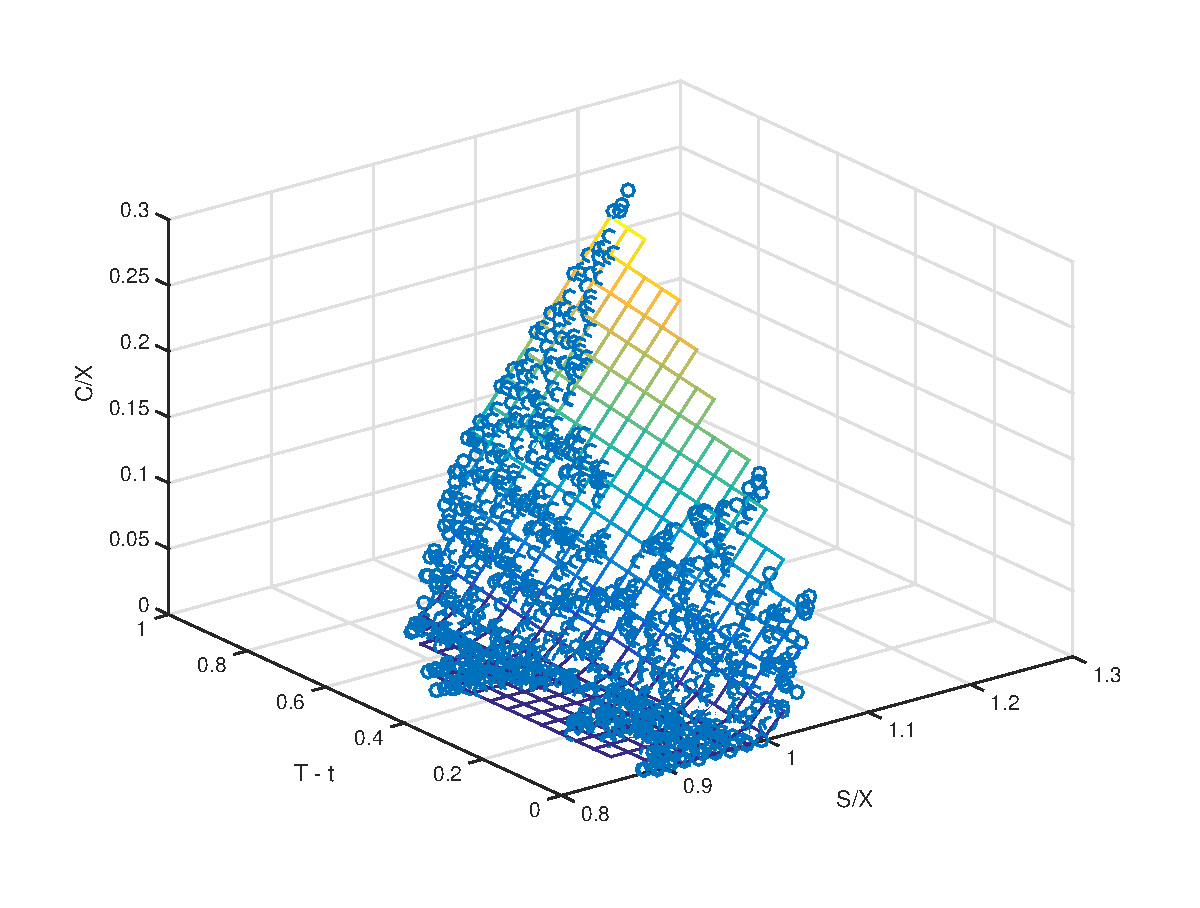
\includegraphics[width=0.75\linewidth]{figures/1.eps}
    \caption{Black-Scholes simulated prices normalized by strike price ($C/X$) and plotted against normalized stock price ($S/X$) and time to expiration ($T - t$)}
    \label{fig:blsprices}
  \end{figure}
  \begin{figure}
    \centering
    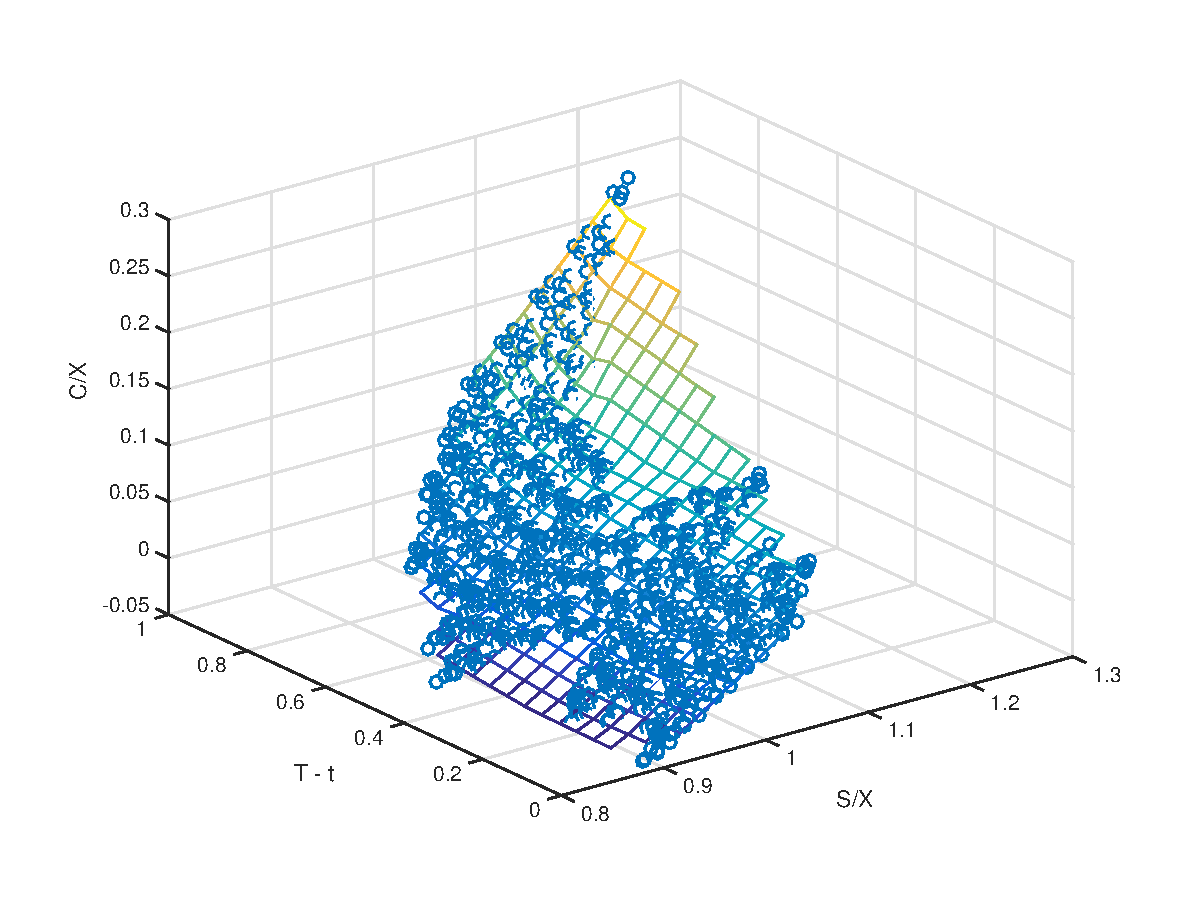
\includegraphics[width=0.75\linewidth]{figures/2.eps}
    \caption{Network call option prices normalized by strike price}
    \label{fig:rdfprices}
  \end{figure}
  \begin{figure}
    \centering
    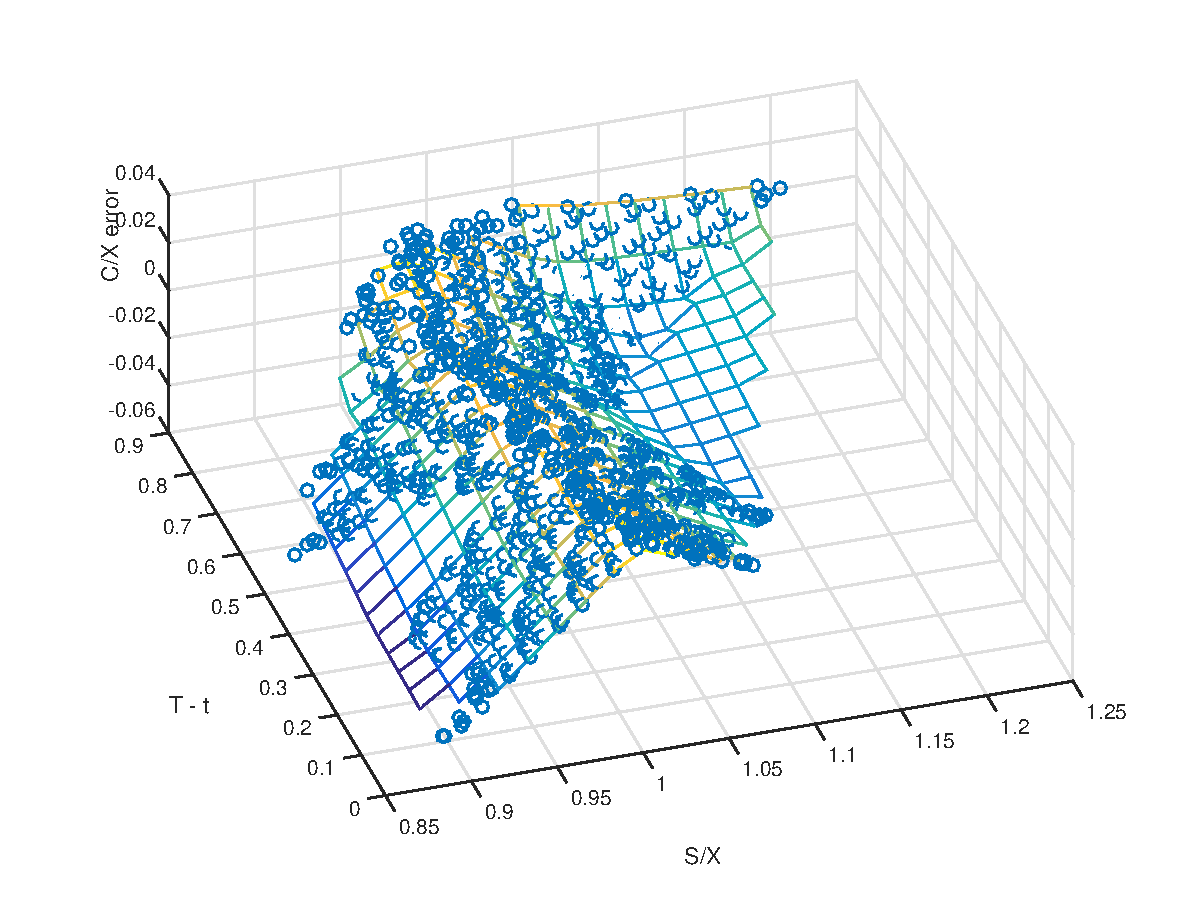
\includegraphics[width=0.75\linewidth]{figures/3.eps}
    \caption{Network call price error}
    \label{fig:rdferror}
  \end{figure}
  \begin{figure}
    \centering
    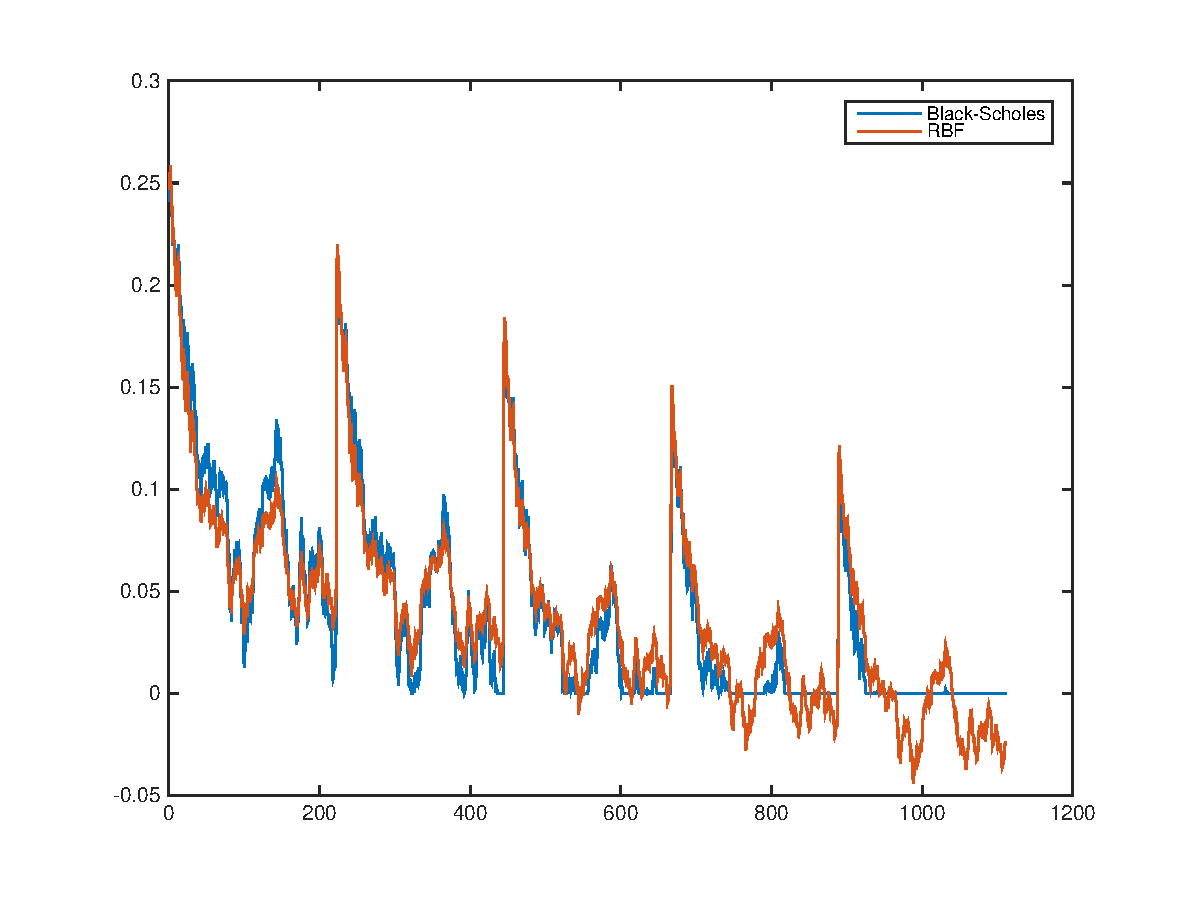
\includegraphics[width=0.75\linewidth]{figures/4.eps}
    \caption{Accuracy of Black-Scholes and RBF models}
    \label{fig:accuracy}
  \end{figure}

  \clearpage
  \appendix

  \section{Code}

  \begin{verbatim}
clear;
load('data.mat');

strike_prices = [ones(222, 1) * 2925; ones(222, 1) * 3025; ones(222, 1) * 3125;
  ones(222, 1) * 3225; ones(222, 1) * 3325];

% Actual prices normalised by strike price (S/X)
actual_prices = [c2925(:, 3) / 2925; c3025(:, 3) / 3025; c3125(:, 3) / 3125;
  c3225(:, 3) / 3225; c3325(:, 3) / 3325];

% Times (T - t)
t = linspace(222 / 252, 0, 222)';
times = [t; t; t; t; t];

prices2925 = c2925(:, 3);
N = size(prices2925, 1);
volatility = std(tick2ret(prices2925, [], 'Continuous')) / sqrt(N / 252);
[call, put] = blsprice(prices2925, 2925, 0.06, t, volatility);
delta2925 = blsdelta(call + 1, 2925, 0.06, t + 1, volatility);
call2925 = call / 2925;

prices3025 = c3025(:, 3);
N = size(prices3025, 1);
volatility = std(tick2ret(prices3025, [], 'Continuous')) / sqrt(N / 252);
[call, put] = blsprice(prices3025, 3025, 0.06, t, volatility);
delta3025 = blsdelta(call + 1, 3025, 0.06, t + 1, volatility);
call3025 = call / 3025;

prices3125 = c3125(:, 3);
N = size(prices3125, 1);
volatility = std(tick2ret(prices3125, [], 'Continuous')) / sqrt(N / 252);
[call, put] = blsprice(prices3125, 3125, 0.06, t, volatility);
delta3125 = blsdelta(call + 1, 3125, 0.06, t + 1, volatility);
call3125 = call / 3125;

prices3225 = c3225(:, 3);
N = size(prices3225, 1);
volatility = std(tick2ret(prices3225, [], 'Continuous')) / sqrt(N / 252);
[call, put] = blsprice(prices3225, 3225, 0.06, t, volatility);
delta3225 = blsdelta(call + 1, 3225, 0.06, t + 1, volatility);
call3225 = call / 3225;

prices3325 = c3325(:, 3);
N = size(prices3325, 1);
volatility = std(tick2ret(prices3325, [], 'Continuous')) / sqrt(N / 252);
[call, put] = blsprice(prices3325, 3325, 0.06, t, volatility);
delta3325 = blsdelta(call + 1, 3325, 0.06, t + 1, volatility);
call3325 = call / 3325;

% Black-Scholes predicted call option prices normalised by strike price
% (C/X)
bls_prices = [call2925; call3025; call3125; call3225; call3325];

bls_deltas = [delta2925; delta3025; delta3125; delta3225; delta3325];

plot_mesh(actual_prices, times, bls_prices);
xlabel('S/X');
ylabel('T - t');
zlabel('C/X');

data = [actual_prices times];
N = size(data, 1);

result = fitgmdist(data, 4, 'Options', statset('MaxIter', 1000));

design_matrix = zeros(N, 7);
design_matrix(:, 7) = ones(N, 1);

design_matrix(:, 5:6) = data;

for j = 1:4
    mean = result.mu(j, :)';
    cov = result.Sigma(:, :, j);
    for n = 1:N
        x = data(n, :)';
        design_matrix(n, j) = sqrt((x - mean)' * cov * (x - mean));
    end
end

w = inv(design_matrix' * design_matrix) * design_matrix' * bls_prices;

rbf_prices = design_matrix * w;

plot_mesh(actual_prices, times, rbf_prices);
xlabel('S/X');
ylabel('T - t');
zlabel('C/X');

plot_mesh(actual_prices, times, rbf_prices - bls_prices(:, 1));
xlabel('S/X');
ylabel('T - t');
zlabel('C/X error');

figure;
plot(bls_prices);
hold on;
plot(rbf_prices);
legend('Black-Scholes', 'RBF');
  \end{verbatim}

  \section{\texttt{plot\_mesh} function}

  \begin{verbatim}
function [] = plot_mesh(X, Y, Z)
  figure;
  F = TriScatteredInterp(X, Y, Z);
  rx = (max(X) - min(X)) / 20;
  ry = (max(Y) - min(Y)) / 20;
  [qx,qy] = meshgrid(min(X):rx:max(X), min(Y):ry:max(Y));
  qz = F(qx,qy);
  mesh(qx,qy,qz);
  hold on;
  scatter3(X, Y, Z);
end
  \end{verbatim}

\end{document}
